\textbf{By understanding the original codes and observing the default plots of this set of data, can you deduce how many times the UAV had taken off and landed?}
\\

The original code provides data on the accelerometer, Euler angles, GPS, and Motor signals, with plots for each aspect. From observing the default plots, only the motor signal plot provides some sort of understanding of how many times the UAV takes off and lands through the 2 input spikes supplied from the motor - observed over different time intervals. The initial GPS plot shown in Figure. (\ref{fig:GPS Plot}), without any processing, is unclear how often the drone takes off and lands. When analyzing the data on the GPS plots, it can be deduced that in the first 32 seconds of the UAV's flight contains an an anomaly in the data. This anomaly, shown through the spike from around 0 m to 1400 m causes a skew in the plot where you are unable to observe the actual movement of the UAV. From the data provided for the flight time, it is clear that 32 seconds falls at around an index of 125, and therefore, a processed GPS plot (code shown in Figure (\ref{fig:GPS Plot Code})) is created as shown in Figure. (\ref{fig:GPS Plot}), where you can see a more clear view of the flight of the UAV. You are able to tell that the \textbf{UAV takes off two times, the first time it flies up by approximately 10 m (1407 m - 1397 m); the second time it flies up by approximately 31 m (1428 m - 1397 m)}.
\\
\begin{minipage}[H]{0.43\textwidth}
    \centering
    % Insert your graph here
    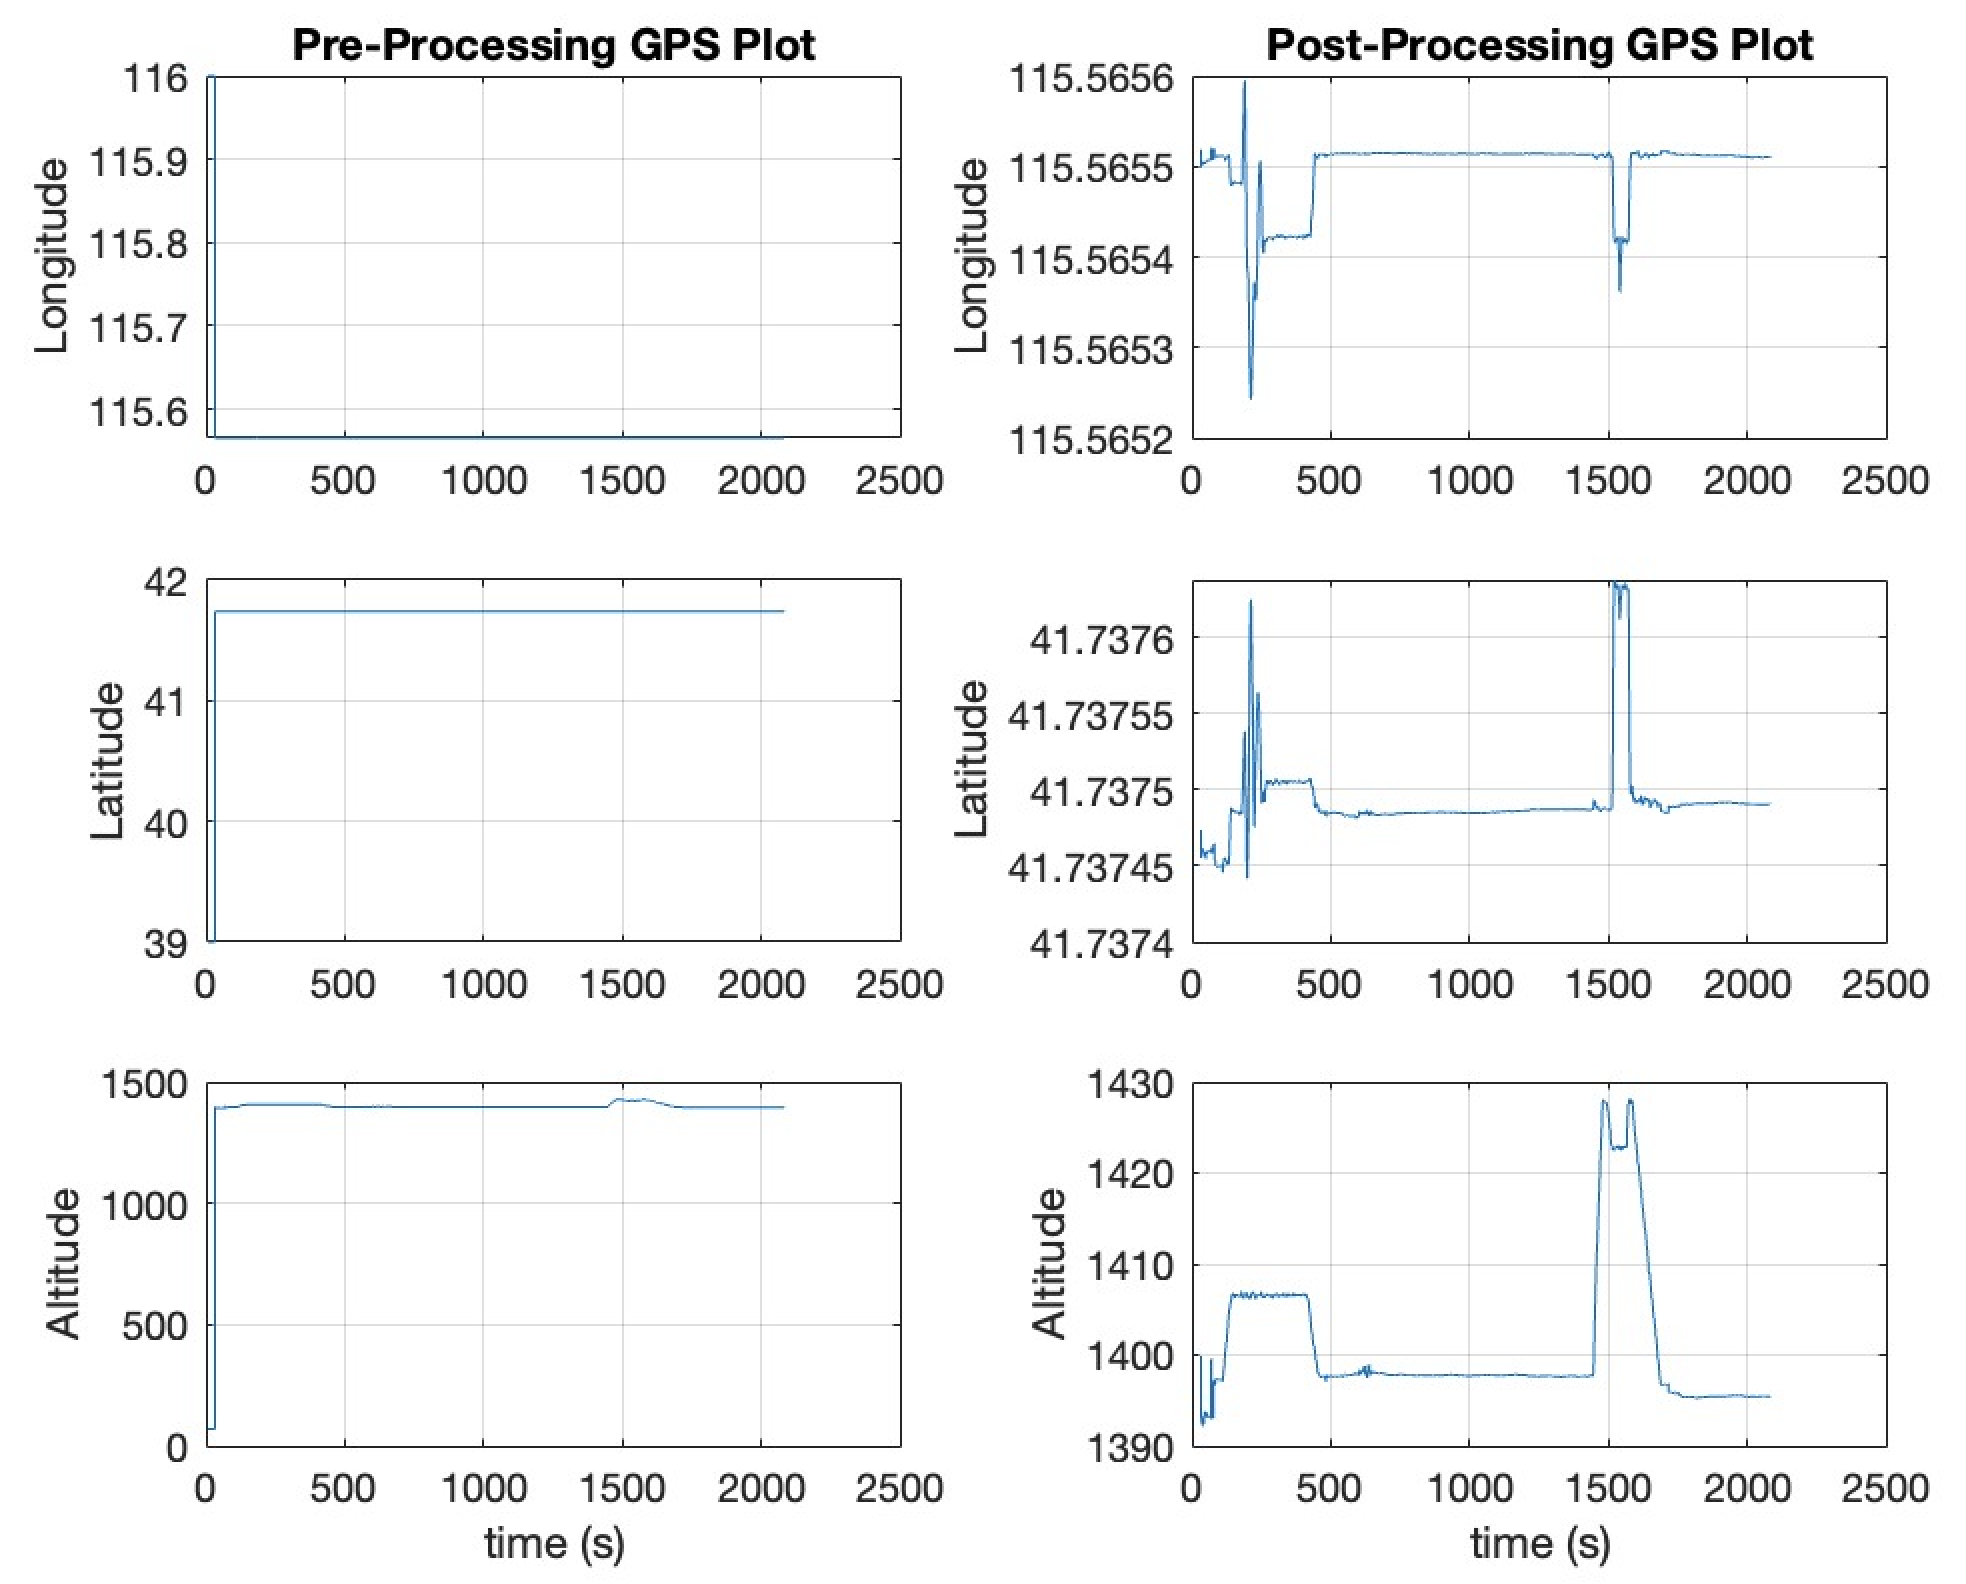
\includegraphics[width=1.6\linewidth]{Introduction/GPS_Plot.png}  
    \label{fig:GPS Plot}
    \captionsetup{justification=centering} % Ensure caption is centered
    \captionof{figure}{Original Code vs. Processed GPS Plot}
\end{minipage}
\hfill
\begin{minipage}{0.3\textwidth}
    \centering
    \lstset{language=Matlab, breaklines=true, basicstyle=\ttfamily\scriptsize}
    \begin{lstlisting}
    
figure; set(gcf,'numbertitle','off','name','GPS');  
subplot(3,2,1); plot(t, lon); title('Pre-Processing GPS Plot'); ylabel('Longitude'); grid on;
subplot(3,2,3); plot(t, lat); ylabel('Latitude'); grid on;
subplot(3,2,5); plot(t, alt); ylabel('Altitude'); grid on; xlabel('time (s)');
subplot(3,2,2); plot(t(125:end), lon(125:end)); title('Post-Processing GPS Plot'); ylabel('Longitude'); grid on;
subplot(3,2,4); plot(t(125:end), lat(125:end)); ylabel('Latitude'); grid on;
subplot(3,2,6); plot(t(125:end), alt(125:end)); ylabel('Altitude'); grid on; xlabel('time (s)');
    \end{lstlisting}
    \captionof{figure}{MATLAB Code for Processed GPS Plot}
    \label{fig:GPS Plot Code}
\end{minipage}


\textbf{}
\\
\textbf{When did the UAV take off and land the second time?}
\\

From Figure. (\ref{fig:GPS Plot}), we can see that the UAV took off the first time at about 113 seconds from when data started to be collected. It was in flight for about 370 seconds, during which point, at 483 seconds, it returned to the base altitude of the UAV of 1397.8 m. \textbf{The UAV took off a second time at about 1443 seconds (24 minutes into flight data being tracked) and was in flight for about 242 seconds when it came back to the base altitude of the UAV at 1685 seconds (28 minutes into flight data being tracked).} The resting state of the UAV can be seen to be at an altitude of around 1397.8 m, which we will take as the UAV being on the ground. Using 1397.8 m as the ground frame measurement, we can capture the time the UAV takes off and lands when we see the base of the 2 spikes in the post-processed altitude graph and the flat line for when the curve returns to our assumed ground frame measurement.